\chapter{Architecture}

This chapter provides an overview of the architecture for the hashing
accelerator and the DMA module designed in the project.

\section{Design of the Hashing Accelerator}

As noted in section \ref{sec:previous-hash}, there are many options for
designing a hashing module. Searching the internet, several existing open-source
implementations of such modules can be found. However, most of these
take advantage of various optimizations which makes the code hard to
read or unsuitable for use in an FPGA.

It was therefore decided to create a new hashing module, using optimizations
only if neccessary, focusing on creating well-written and easy-to-read source
code that can later be easily extended or modified.

To do this, a simple module was constructed that runs one iteration of
the compression function each cycle, calculating the hash of one block
of data in 64 cycles with an additional cycle added for creating the
final hash from the intermediate values from the previous round (see
section \ref{sec:hashing-algo} for details).

Using no optimizations yielded a hashing accelerator module that can
run at approximately 50~MHz, the same clock frequency as used in the SHMAC system.
Because of this, and in order to preserve the readability of the code, it
was decided not to attempt to improve the performance of the module.

\subsection{Theoretical Maximum Performance}
If the hashing module can finish hashing a block of data in 65 cycles and
every hash can be obtained from only one block of data, it is possible to
obtain a finished hash every 65 clock cycles under ideal conditions. This
translates into a maximum theoretical performance of 768230~H/s at a clock
frequency of 50~MHz.

However, in real-life, the modules do not exist in a vacuum, and data needs to be transferred
between the modules and a controller, such as a microprocessor. If the hashing tiles
are connected to the rest of the system using an AXI4 lite interface, transfers
takes at least three cycles for writes and two cycles for reads.
It is assumed that no burst transfers are used and that only one transaction
can be executed at a time, corresponding with the requirements for the interface.

In order for the hashing module to work, it needs 16 32-bit words of input data,
and control signals must be set up. This causes at least 17 words of data to
need to be written to the module, taking at least 51 clock cycles. Then, after
hashing of a block is complete, if there are no more blocks, the result must
be read back. The result consists of 8 words of data, which takes at least 16
clock cycles to transfer.

In total, a minimum of 67 clock cycles of overhead is needed per hash when assuming
a one-block input size and an ideal AXI4 bus. Not considering the additional overhead
from processing in the microprocessor, such as when handlig the interrupt when the
hashing finishes, hashing may take a minimum of $67 + 65 = 132$ clock cycles to
complete, bringing the maximum theoretical performance down to at most 378787~H/s.

\section{Design of the DMA Module}
\label{sec:dma-architecture}

\subsection{Assumptions}
To simplify the design of the DMA module, some assumptions as to the system where the
DMA is implemented needs to be done.

It is assumed that all data is transferred sequentially. 
This is especially important when it comes to future integration into the SHMAC system, because of the XY routing that the system uses.
However, such an assumption also significantly simplifies the design of the DMA for use in shared-bus systems.

Any issues regarding virtual memory and cache coherency are assumed to be handled outside the DMA module.

%\subsection{Design requirements}
\subsection{Chosen functionality in design}

It was decided on a couple of requirements for the DMA implementation.

\begin{description}
	\item[Use block-to-block transfers.] This is a minimum requirement for being
	able to transfer any amount of data from locations A to B.
	\item[Two channels.] This allows the DMA to have two separate transfers going
	at the same time.
	The number of channels is inspired by the Adapteva Epiphany \cite{epiphany}, where every DMA module has two generic channel each.
	With a high number of DMA modules, a high number of channels in each DMA module is not necessary.
	\item[Automatic channel allocation.] Channel allocation is done in hardware,
	saving the CPU from the overhead of allocating and managing channels in software.
	\item[Buffer containing multiple requests] Inspired by the Cell multiprocessor.
	If more advanced versions of the DMA module, implemented in SHMAC, is to be able to handle multiple requests and of different types, issued by more than one source, then a buffer to receive and queue these requests is useful.
	% I removed component-based implementation, because _every_ hardware design is component based. -K.
	% 
	% Yeah.... that makes sense. You should have taken TFE4140 last spring, not every student though of component based design, as they threw together a lot of code at top-level :-P
\end{description}

\subsection{DMA Architecture}

The DMA module consists of several main components: a FIFO buffer that contains transfer requests from the CPU, a main controller that processes the requests and delegate them to the channels, and two channels where the memory transfers are executed.
The two channels work on independent transfer tasks.
An arbiter is used to control access to the bus interface for the two channels and the DMA Controller, with interrupt signals from the DMA Controller having highest priority, followed by storing commands and then loading commands.
Another FIFO buffer is used to receive and queue loaded data.
The loaded data is compared with the requested data from the channels by checking if their addresses match. 
An overview of the DMA architecture can be seen in figure \ref{fig:DMATopView2}.
The overview provided in this chapter is simplified.
For more details, see appendix \ref{app:DMA-arch}.

\begin{figure}[htb]
    \centering
    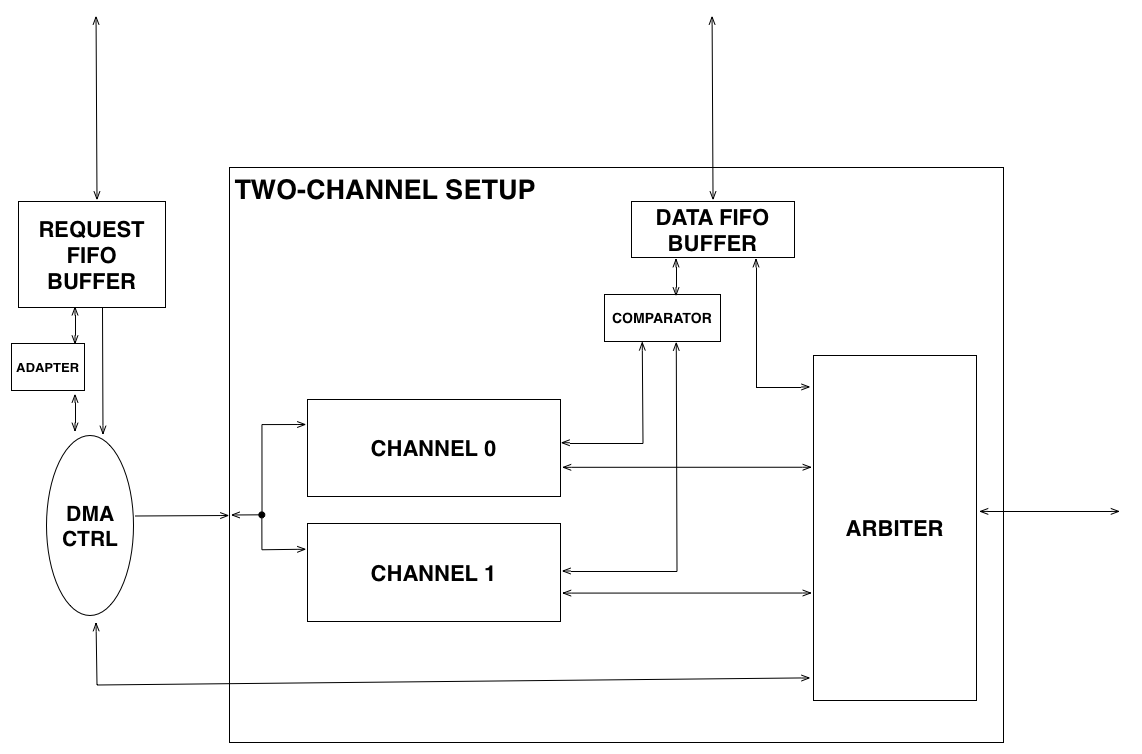
\includegraphics[width=1\textwidth]{Figures/DMA/TopViewFinalSimple2}
    \caption{DMA module overview. }
    \label{fig:DMATopView2}
\end{figure}

\subsubsection{Main Controller}
The role of the main controller is to process incoming transfer requests, allocate and activate
channels that are free to execute requests, monitor the channels, and send out an interrupt signal
when a transfer is completed.
The controller is implemented as a state machine, shown in figure \ref{fig:DMAControllerStateMachineSimple2}.

\begin{figure}[htb]
    \centering
    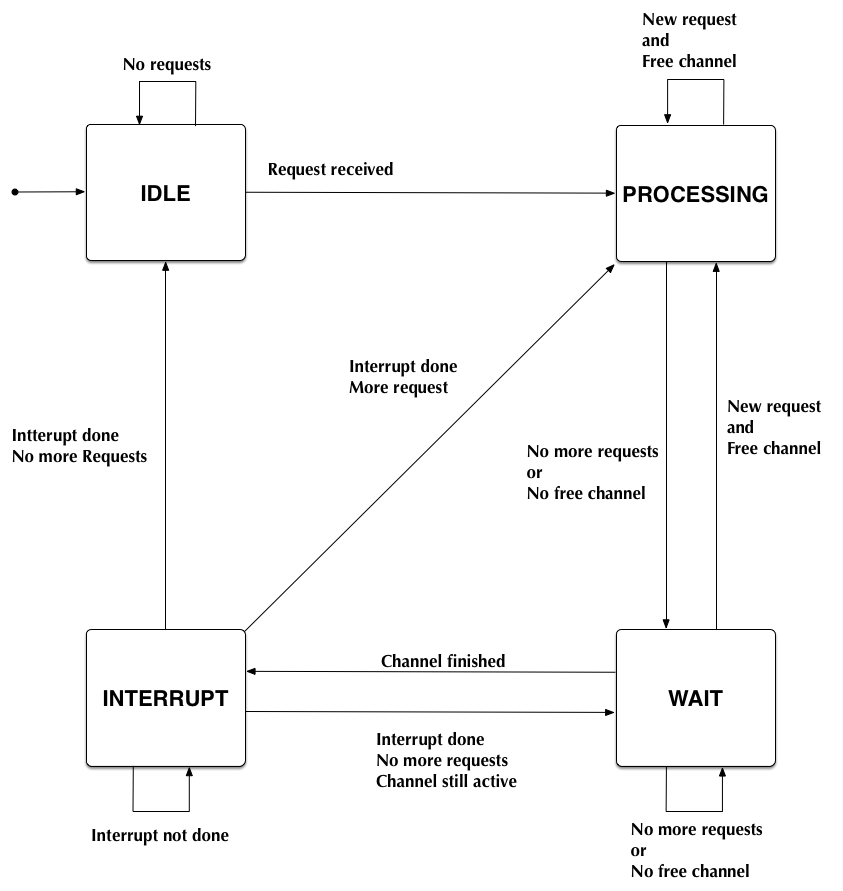
\includegraphics[width=1\textwidth]{Figures/DMA/StateMachineFinalSimple}
    \caption{DMA Controller State Machine}
    \label{fig:DMAControllerStateMachineSimple2}
\end{figure}

% IMPORTANT: Before you start talking about being too detailed, Kristian, my group got slaugthered in Computer Architecture project (TDT4260) for showing figures in result section without explaining them in the text. Do not count on figures to be self-explanatory. 
Four states are used: IDLE; PROCESSING, WAIT and INTERRUPT.
Whenever there is no activity and no incoming tranfer request, the state is IDLE.
When activating a new channel for a requested transfer, the state is PROCESSING. 
There must be a request to handle, and at least a free channel to jump to this state from any other state.
When at least one channel is active, the state is WAIT as long as no more channels can be activated (either due to no more requests or all channels already being active).
When sending out interrupt signal, the state is INTERRUPT.

\subsubsection{Channels}
Each channel is split into two parts: a part that is responsible for sending out load
commands, and a storing part that issues store commands when associated data has arrived. 
These ``subchannels'' are called the load channel and store channel, respectively.
They are not to be confused with channels 0 and 1 that are shown in figure \ref{fig:DMATopView2}.
Both channels have a load channel and a store channel each.

\subsubsection{Bus interaction system}
\todo{Kristian: Is master interface and slave interface covered well enough in the appendix?}In order for the DMA module to be as general as possible, it contains only a generic
interface for communicating with a bus system. An adapter is then used to connect
the module to the bus system. This makes it possible to connect the DMA module to
different kinds of busses by simply writing an adapter for the desired system.

\subsubsection{Running the DMA Module}
\todo{Kristian: Jeg husker Yaman etterlyste dette. Finnes på 3.1.2. fra hans første tilbakemelding. Så langt jeg vet har du bedre oversikt på denne enn jeg}
TODO:
Yaman skrev dette på 3.1.2. på første tilbakemelding:

"consider adding a small section describing what a DMA transfer looks like end-to-end, e.g how the CPU sets up the transfer, how DMA executes it and the CPU gets notified. 

also make sure to underline that the way transfer requests are made is different then the traditional memory-mapped control registers with channel allocation completely managed in software."
